% Created by tikzDevice version 0.12.6 on 2024-04-16 16:15:50
% !TEX encoding = UTF-8 Unicode
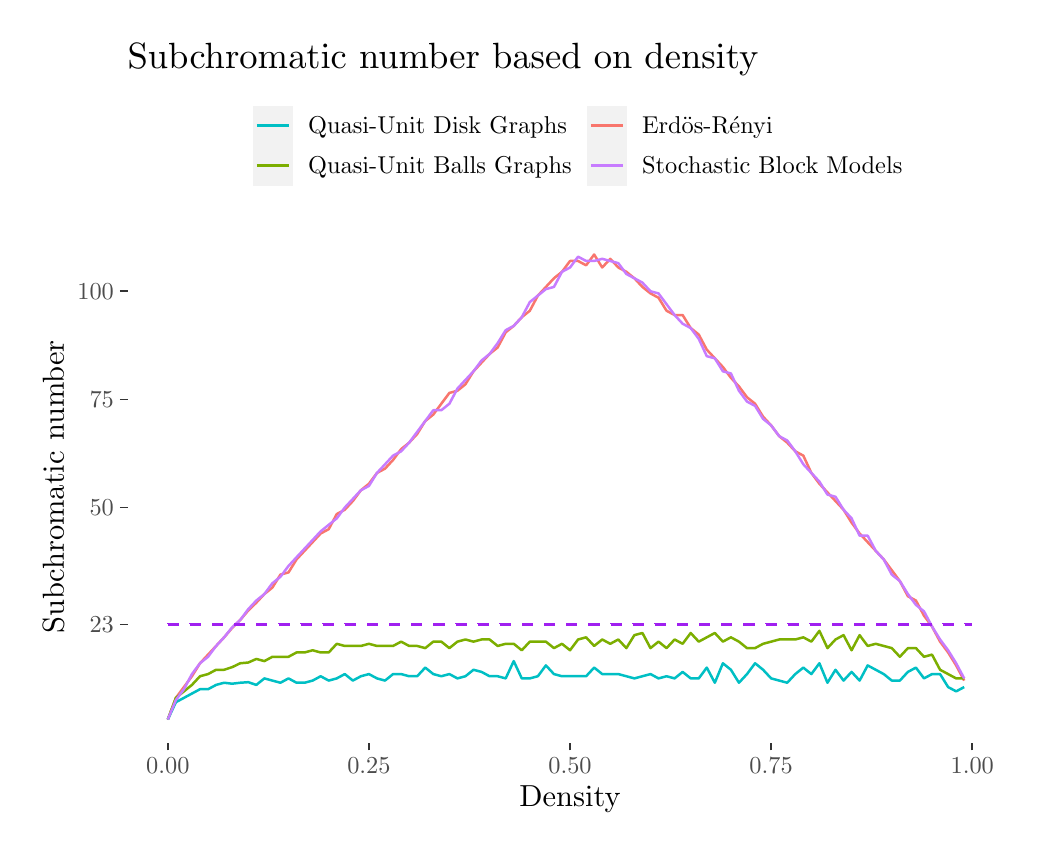
\begin{tikzpicture}[x=1pt,y=1pt]
\definecolor{fillColor}{RGB}{255,255,255}
\path[use as bounding box,fill=fillColor,fill opacity=0.00] (0,0) rectangle (361.35,289.08);
\begin{scope}
\path[clip] (  0.00,  0.00) rectangle (361.35,289.08);
\definecolor{drawColor}{RGB}{255,255,255}
\definecolor{fillColor}{RGB}{255,255,255}

\path[draw=drawColor,line width= 0.6pt,line join=round,line cap=round,fill=fillColor] (  0.00,  0.00) rectangle (361.35,289.08);
\end{scope}
\begin{scope}
\path[clip] ( 36.11, 30.69) rectangle (355.85,215.51);
\definecolor{fillColor}{RGB}{255,255,255}

\path[fill=fillColor] ( 36.11, 30.69) rectangle (355.85,215.51);
\definecolor{drawColor}{RGB}{248,118,109}

\path[draw=drawColor,line width= 0.9pt,line join=round] ( 50.64, 39.09) --
	( 53.55, 46.90) --
	( 56.46, 50.81) --
	( 59.36, 54.72) --
	( 62.27, 59.41) --
	( 65.18, 62.53) --
	( 68.09, 65.66) --
	( 70.99, 68.78) --
	( 73.90, 72.19) --
	( 76.81, 75.04) --
	( 79.71, 78.48) --
	( 82.62, 81.29) --
	( 85.53, 84.42) --
	( 88.43, 86.76) --
	( 91.34, 91.45) --
	( 94.25, 92.23) --
	( 97.15, 96.92) --
	(100.06,100.05) --
	(102.97,103.17) --
	(105.87,106.30) --
	(108.78,107.86) --
	(111.69,113.33) --
	(114.59,114.89) --
	(117.50,118.02) --
	(120.41,121.93) --
	(123.31,124.27) --
	(126.22,128.18) --
	(129.13,129.74) --
	(132.03,132.87) --
	(134.94,136.78) --
	(137.85,139.12) --
	(140.75,142.25) --
	(143.66,146.94) --
	(146.57,149.28) --
	(149.47,153.19) --
	(152.38,157.10) --
	(155.29,157.88) --
	(158.19,160.22) --
	(161.10,164.91) --
	(164.01,168.04) --
	(166.91,171.16) --
	(169.82,173.51) --
	(172.73,178.98) --
	(175.63,181.32) --
	(178.54,184.45) --
	(181.45,186.79) --
	(184.35,192.26) --
	(187.26,195.39) --
	(190.17,198.52) --
	(193.07,200.86) --
	(195.98,204.77) --
	(198.89,204.77) --
	(201.79,203.21) --
	(204.70,207.11) --
	(207.61,202.42) --
	(210.51,205.55) --
	(213.42,202.42) --
	(216.33,200.86) --
	(219.23,198.52) --
	(222.14,195.39) --
	(225.05,193.05) --
	(227.95,191.48) --
	(230.86,186.79) --
	(233.77,185.23) --
	(236.67,185.23) --
	(239.58,180.54) --
	(242.49,178.20) --
	(245.39,172.73) --
	(248.30,169.60) --
	(251.21,166.47) --
	(254.11,162.57) --
	(257.02,159.44) --
	(259.93,155.53) --
	(262.84,153.19) --
	(265.74,148.50) --
	(268.65,145.37) --
	(271.56,141.47) --
	(274.46,139.12) --
	(277.37,136.00) --
	(280.28,134.43) --
	(283.18,128.18) --
	(286.09,124.27) --
	(289.00,121.15) --
	(291.90,118.02) --
	(294.81,114.89) --
	(297.72,110.21) --
	(300.62,106.30) --
	(303.53,103.17) --
	(306.44,100.05) --
	(309.34, 96.92) --
	(312.25, 93.01) --
	(315.16, 89.10) --
	(318.06, 83.63) --
	(320.97, 82.07) --
	(323.88, 76.60) --
	(326.78, 72.69) --
	(329.69, 67.22) --
	(332.60, 63.31) --
	(335.50, 58.63) --
	(338.41, 53.15);
\definecolor{drawColor}{RGB}{124,174,0}

\path[draw=drawColor,line width= 0.9pt,line join=round] ( 50.64, 39.09) --
	( 53.55, 46.90) --
	( 56.46, 49.25) --
	( 59.36, 51.59) --
	( 62.27, 54.72) --
	( 65.18, 55.50) --
	( 68.09, 57.06) --
	( 70.99, 57.06) --
	( 73.90, 58.01) --
	( 76.81, 59.41) --
	( 79.71, 59.67) --
	( 82.62, 60.97) --
	( 85.53, 60.19) --
	( 88.43, 61.75) --
	( 91.34, 61.75) --
	( 94.25, 61.75) --
	( 97.15, 63.31) --
	(100.06, 63.31) --
	(102.97, 64.10) --
	(105.87, 63.31) --
	(108.78, 63.31) --
	(111.69, 66.44) --
	(114.59, 65.66) --
	(117.50, 65.66) --
	(120.41, 65.66) --
	(123.31, 66.44) --
	(126.22, 65.66) --
	(129.13, 65.66) --
	(132.03, 65.66) --
	(134.94, 67.22) --
	(137.85, 65.66) --
	(140.75, 65.66) --
	(143.66, 64.88) --
	(146.57, 67.22) --
	(149.47, 67.22) --
	(152.38, 64.88) --
	(155.29, 67.22) --
	(158.19, 68.00) --
	(161.10, 67.22) --
	(164.01, 68.00) --
	(166.91, 68.00) --
	(169.82, 65.66) --
	(172.73, 66.44) --
	(175.63, 66.44) --
	(178.54, 64.10) --
	(181.45, 67.22) --
	(184.35, 67.22) --
	(187.26, 67.22) --
	(190.17, 64.88) --
	(193.07, 66.44) --
	(195.98, 64.10) --
	(198.89, 68.00) --
	(201.79, 68.78) --
	(204.70, 65.66) --
	(207.61, 68.00) --
	(210.51, 66.44) --
	(213.42, 68.00) --
	(216.33, 64.88) --
	(219.23, 69.57) --
	(222.14, 70.35) --
	(225.05, 64.88) --
	(227.95, 67.22) --
	(230.86, 64.88) --
	(233.77, 68.00) --
	(236.67, 66.44) --
	(239.58, 70.35) --
	(242.49, 67.22) --
	(245.39, 68.78) --
	(248.30, 70.35) --
	(251.21, 67.22) --
	(254.11, 68.78) --
	(257.02, 67.22) --
	(259.93, 64.88) --
	(262.84, 64.88) --
	(265.74, 66.44) --
	(268.65, 67.22) --
	(271.56, 68.00) --
	(274.46, 68.00) --
	(277.37, 68.00) --
	(280.28, 68.78) --
	(283.18, 67.22) --
	(286.09, 71.13) --
	(289.00, 64.88) --
	(291.90, 68.00) --
	(294.81, 69.57) --
	(297.72, 64.10) --
	(300.62, 69.57) --
	(303.53, 65.66) --
	(306.44, 66.44) --
	(309.34, 65.66) --
	(312.25, 64.88) --
	(315.16, 61.75) --
	(318.06, 64.88) --
	(320.97, 64.88) --
	(323.88, 61.75) --
	(326.78, 62.53) --
	(329.69, 57.06) --
	(332.60, 55.50) --
	(335.50, 53.94) --
	(338.41, 53.94);
\definecolor{drawColor}{RGB}{0,191,196}

\path[draw=drawColor,line width= 0.9pt,line join=round] ( 50.64, 39.09) --
	( 53.55, 45.34) --
	( 56.46, 46.90) --
	( 59.36, 48.47) --
	( 62.27, 50.03) --
	( 65.18, 50.03) --
	( 68.09, 51.59) --
	( 70.99, 52.37) --
	( 73.90, 52.02) --
	( 76.81, 52.37) --
	( 79.71, 52.57) --
	( 82.62, 51.59) --
	( 85.53, 53.94) --
	( 88.43, 53.15) --
	( 91.34, 52.37) --
	( 94.25, 53.94) --
	( 97.15, 52.37) --
	(100.06, 52.37) --
	(102.97, 53.15) --
	(105.87, 54.72) --
	(108.78, 53.15) --
	(111.69, 53.94) --
	(114.59, 55.50) --
	(117.50, 53.15) --
	(120.41, 54.72) --
	(123.31, 55.50) --
	(126.22, 53.94) --
	(129.13, 53.15) --
	(132.03, 55.50) --
	(134.94, 55.50) --
	(137.85, 54.72) --
	(140.75, 54.72) --
	(143.66, 57.84) --
	(146.57, 55.50) --
	(149.47, 54.72) --
	(152.38, 55.50) --
	(155.29, 53.94) --
	(158.19, 54.72) --
	(161.10, 57.06) --
	(164.01, 56.28) --
	(166.91, 54.72) --
	(169.82, 54.72) --
	(172.73, 53.94) --
	(175.63, 60.19) --
	(178.54, 53.94) --
	(181.45, 53.94) --
	(184.35, 54.72) --
	(187.26, 58.63) --
	(190.17, 55.50) --
	(193.07, 54.72) --
	(195.98, 54.72) --
	(198.89, 54.72) --
	(201.79, 54.72) --
	(204.70, 57.84) --
	(207.61, 55.50) --
	(210.51, 55.50) --
	(213.42, 55.50) --
	(216.33, 54.72) --
	(219.23, 53.94) --
	(222.14, 54.72) --
	(225.05, 55.50) --
	(227.95, 53.94) --
	(230.86, 54.72) --
	(233.77, 53.94) --
	(236.67, 56.28) --
	(239.58, 53.94) --
	(242.49, 53.94) --
	(245.39, 57.84) --
	(248.30, 52.37) --
	(251.21, 59.41) --
	(254.11, 57.06) --
	(257.02, 52.37) --
	(259.93, 55.50) --
	(262.84, 59.41) --
	(265.74, 57.06) --
	(268.65, 53.94) --
	(271.56, 53.15) --
	(274.46, 52.37) --
	(277.37, 55.50) --
	(280.28, 57.84) --
	(283.18, 55.50) --
	(286.09, 59.41) --
	(289.00, 52.37) --
	(291.90, 57.06) --
	(294.81, 53.15) --
	(297.72, 56.28) --
	(300.62, 53.15) --
	(303.53, 58.63) --
	(306.44, 57.06) --
	(309.34, 55.50) --
	(312.25, 53.15) --
	(315.16, 53.15) --
	(318.06, 56.28) --
	(320.97, 57.84) --
	(323.88, 53.94) --
	(326.78, 55.50) --
	(329.69, 55.50) --
	(332.60, 50.81) --
	(335.50, 49.25) --
	(338.41, 50.81);
\definecolor{drawColor}{RGB}{199,124,255}

\path[draw=drawColor,line width= 0.9pt,line join=round] ( 50.64, 39.09) --
	( 53.55, 46.12) --
	( 56.46, 50.03) --
	( 59.36, 55.50) --
	( 62.27, 59.41) --
	( 65.18, 61.75) --
	( 68.09, 65.66) --
	( 70.99, 68.78) --
	( 73.90, 72.39) --
	( 76.81, 75.04) --
	( 79.71, 78.96) --
	( 82.62, 82.07) --
	( 85.53, 84.42) --
	( 88.43, 88.32) --
	( 91.34, 90.67) --
	( 94.25, 94.57) --
	( 97.15, 97.70) --
	(100.06,100.83) --
	(102.97,103.95) --
	(105.87,107.08) --
	(108.78,109.42) --
	(111.69,111.77) --
	(114.59,115.68) --
	(117.50,118.80) --
	(120.41,121.93) --
	(123.31,123.49) --
	(126.22,128.18) --
	(129.13,131.31) --
	(132.03,134.43) --
	(134.94,136.00) --
	(137.85,139.12) --
	(140.75,143.03) --
	(143.66,146.94) --
	(146.57,150.84) --
	(149.47,150.84) --
	(152.38,153.19) --
	(155.29,158.66) --
	(158.19,161.79) --
	(161.10,164.91) --
	(164.01,168.82) --
	(166.91,171.16) --
	(169.82,175.07) --
	(172.73,179.76) --
	(175.63,181.32) --
	(178.54,184.45) --
	(181.45,189.92) --
	(184.35,192.26) --
	(187.26,194.61) --
	(190.17,195.39) --
	(193.07,200.86) --
	(195.98,202.42) --
	(198.89,206.33) --
	(201.79,204.77) --
	(204.70,204.77) --
	(207.61,205.55) --
	(210.51,204.77) --
	(213.42,203.99) --
	(216.33,200.08) --
	(219.23,198.52) --
	(222.14,196.95) --
	(225.05,193.83) --
	(227.95,193.05) --
	(230.86,189.14) --
	(233.77,185.23) --
	(236.67,182.10) --
	(239.58,180.54) --
	(242.49,176.63) --
	(245.39,170.38) --
	(248.30,169.60) --
	(251.21,164.91) --
	(254.11,164.13) --
	(257.02,157.88) --
	(259.93,153.97) --
	(262.84,152.41) --
	(265.74,147.72) --
	(268.65,145.37) --
	(271.56,141.47) --
	(274.46,139.90) --
	(277.37,136.00) --
	(280.28,131.31) --
	(283.18,128.18) --
	(286.09,125.05) --
	(289.00,120.36) --
	(291.90,119.58) --
	(294.81,114.89) --
	(297.72,111.77) --
	(300.62,105.52) --
	(303.53,105.52) --
	(306.44,100.05) --
	(309.34, 96.92) --
	(312.25, 91.45) --
	(315.16, 89.10) --
	(318.06, 84.42) --
	(320.97, 80.51) --
	(323.88, 78.16) --
	(326.78, 72.69) --
	(329.69, 68.00) --
	(332.60, 64.10) --
	(335.50, 59.41) --
	(338.41, 53.94);
\definecolor{drawColor}{RGB}{160,32,240}

\path[draw=drawColor,line width= 0.9pt,dash pattern=on 4pt off 4pt ,line join=round] ( 50.64, 73.47) -- (341.32, 73.47);

\path[draw=drawColor,line width= 0.9pt,dash pattern=on 4pt off 4pt ,line join=round] ( 50.64, 73.47) -- (341.32, 73.47);

\path[draw=drawColor,line width= 0.9pt,dash pattern=on 4pt off 4pt ,line join=round] ( 50.64, 73.47) -- (341.32, 73.47);

\path[draw=drawColor,line width= 0.9pt,dash pattern=on 4pt off 4pt ,line join=round] ( 50.64, 73.47) -- (341.32, 73.47);

\path[draw=drawColor,line width= 0.9pt,dash pattern=on 4pt off 4pt ,line join=round] ( 50.64, 73.47) -- (341.32, 73.47);

\path[draw=drawColor,line width= 0.9pt,dash pattern=on 4pt off 4pt ,line join=round] ( 50.64, 73.47) -- (341.32, 73.47);

\path[draw=drawColor,line width= 0.9pt,dash pattern=on 4pt off 4pt ,line join=round] ( 50.64, 73.47) -- (341.32, 73.47);

\path[draw=drawColor,line width= 0.9pt,dash pattern=on 4pt off 4pt ,line join=round] ( 50.64, 73.47) -- (341.32, 73.47);

\path[draw=drawColor,line width= 0.9pt,dash pattern=on 4pt off 4pt ,line join=round] ( 50.64, 73.47) -- (341.32, 73.47);

\path[draw=drawColor,line width= 0.9pt,dash pattern=on 4pt off 4pt ,line join=round] ( 50.64, 73.47) -- (341.32, 73.47);

\path[draw=drawColor,line width= 0.9pt,dash pattern=on 4pt off 4pt ,line join=round] ( 50.64, 73.47) -- (341.32, 73.47);

\path[draw=drawColor,line width= 0.9pt,dash pattern=on 4pt off 4pt ,line join=round] ( 50.64, 73.47) -- (341.32, 73.47);

\path[draw=drawColor,line width= 0.9pt,dash pattern=on 4pt off 4pt ,line join=round] ( 50.64, 73.47) -- (341.32, 73.47);

\path[draw=drawColor,line width= 0.9pt,dash pattern=on 4pt off 4pt ,line join=round] ( 50.64, 73.47) -- (341.32, 73.47);

\path[draw=drawColor,line width= 0.9pt,dash pattern=on 4pt off 4pt ,line join=round] ( 50.64, 73.47) -- (341.32, 73.47);

\path[draw=drawColor,line width= 0.9pt,dash pattern=on 4pt off 4pt ,line join=round] ( 50.64, 73.47) -- (341.32, 73.47);

\path[draw=drawColor,line width= 0.9pt,dash pattern=on 4pt off 4pt ,line join=round] ( 50.64, 73.47) -- (341.32, 73.47);

\path[draw=drawColor,line width= 0.9pt,dash pattern=on 4pt off 4pt ,line join=round] ( 50.64, 73.47) -- (341.32, 73.47);

\path[draw=drawColor,line width= 0.9pt,dash pattern=on 4pt off 4pt ,line join=round] ( 50.64, 73.47) -- (341.32, 73.47);

\path[draw=drawColor,line width= 0.9pt,dash pattern=on 4pt off 4pt ,line join=round] ( 50.64, 73.47) -- (341.32, 73.47);

\path[draw=drawColor,line width= 0.9pt,dash pattern=on 4pt off 4pt ,line join=round] ( 50.64, 73.47) -- (341.32, 73.47);

\path[draw=drawColor,line width= 0.9pt,dash pattern=on 4pt off 4pt ,line join=round] ( 50.64, 73.47) -- (341.32, 73.47);

\path[draw=drawColor,line width= 0.9pt,dash pattern=on 4pt off 4pt ,line join=round] ( 50.64, 73.47) -- (341.32, 73.47);

\path[draw=drawColor,line width= 0.9pt,dash pattern=on 4pt off 4pt ,line join=round] ( 50.64, 73.47) -- (341.32, 73.47);

\path[draw=drawColor,line width= 0.9pt,dash pattern=on 4pt off 4pt ,line join=round] ( 50.64, 73.47) -- (341.32, 73.47);

\path[draw=drawColor,line width= 0.9pt,dash pattern=on 4pt off 4pt ,line join=round] ( 50.64, 73.47) -- (341.32, 73.47);

\path[draw=drawColor,line width= 0.9pt,dash pattern=on 4pt off 4pt ,line join=round] ( 50.64, 73.47) -- (341.32, 73.47);

\path[draw=drawColor,line width= 0.9pt,dash pattern=on 4pt off 4pt ,line join=round] ( 50.64, 73.47) -- (341.32, 73.47);

\path[draw=drawColor,line width= 0.9pt,dash pattern=on 4pt off 4pt ,line join=round] ( 50.64, 73.47) -- (341.32, 73.47);

\path[draw=drawColor,line width= 0.9pt,dash pattern=on 4pt off 4pt ,line join=round] ( 50.64, 73.47) -- (341.32, 73.47);

\path[draw=drawColor,line width= 0.9pt,dash pattern=on 4pt off 4pt ,line join=round] ( 50.64, 73.47) -- (341.32, 73.47);

\path[draw=drawColor,line width= 0.9pt,dash pattern=on 4pt off 4pt ,line join=round] ( 50.64, 73.47) -- (341.32, 73.47);

\path[draw=drawColor,line width= 0.9pt,dash pattern=on 4pt off 4pt ,line join=round] ( 50.64, 73.47) -- (341.32, 73.47);

\path[draw=drawColor,line width= 0.9pt,dash pattern=on 4pt off 4pt ,line join=round] ( 50.64, 73.47) -- (341.32, 73.47);

\path[draw=drawColor,line width= 0.9pt,dash pattern=on 4pt off 4pt ,line join=round] ( 50.64, 73.47) -- (341.32, 73.47);

\path[draw=drawColor,line width= 0.9pt,dash pattern=on 4pt off 4pt ,line join=round] ( 50.64, 73.47) -- (341.32, 73.47);

\path[draw=drawColor,line width= 0.9pt,dash pattern=on 4pt off 4pt ,line join=round] ( 50.64, 73.47) -- (341.32, 73.47);

\path[draw=drawColor,line width= 0.9pt,dash pattern=on 4pt off 4pt ,line join=round] ( 50.64, 73.47) -- (341.32, 73.47);

\path[draw=drawColor,line width= 0.9pt,dash pattern=on 4pt off 4pt ,line join=round] ( 50.64, 73.47) -- (341.32, 73.47);

\path[draw=drawColor,line width= 0.9pt,dash pattern=on 4pt off 4pt ,line join=round] ( 50.64, 73.47) -- (341.32, 73.47);

\path[draw=drawColor,line width= 0.9pt,dash pattern=on 4pt off 4pt ,line join=round] ( 50.64, 73.47) -- (341.32, 73.47);

\path[draw=drawColor,line width= 0.9pt,dash pattern=on 4pt off 4pt ,line join=round] ( 50.64, 73.47) -- (341.32, 73.47);

\path[draw=drawColor,line width= 0.9pt,dash pattern=on 4pt off 4pt ,line join=round] ( 50.64, 73.47) -- (341.32, 73.47);

\path[draw=drawColor,line width= 0.9pt,dash pattern=on 4pt off 4pt ,line join=round] ( 50.64, 73.47) -- (341.32, 73.47);

\path[draw=drawColor,line width= 0.9pt,dash pattern=on 4pt off 4pt ,line join=round] ( 50.64, 73.47) -- (341.32, 73.47);

\path[draw=drawColor,line width= 0.9pt,dash pattern=on 4pt off 4pt ,line join=round] ( 50.64, 73.47) -- (341.32, 73.47);

\path[draw=drawColor,line width= 0.9pt,dash pattern=on 4pt off 4pt ,line join=round] ( 50.64, 73.47) -- (341.32, 73.47);

\path[draw=drawColor,line width= 0.9pt,dash pattern=on 4pt off 4pt ,line join=round] ( 50.64, 73.47) -- (341.32, 73.47);

\path[draw=drawColor,line width= 0.9pt,dash pattern=on 4pt off 4pt ,line join=round] ( 50.64, 73.47) -- (341.32, 73.47);

\path[draw=drawColor,line width= 0.9pt,dash pattern=on 4pt off 4pt ,line join=round] ( 50.64, 73.47) -- (341.32, 73.47);

\path[draw=drawColor,line width= 0.9pt,dash pattern=on 4pt off 4pt ,line join=round] ( 50.64, 73.47) -- (341.32, 73.47);

\path[draw=drawColor,line width= 0.9pt,dash pattern=on 4pt off 4pt ,line join=round] ( 50.64, 73.47) -- (341.32, 73.47);

\path[draw=drawColor,line width= 0.9pt,dash pattern=on 4pt off 4pt ,line join=round] ( 50.64, 73.47) -- (341.32, 73.47);

\path[draw=drawColor,line width= 0.9pt,dash pattern=on 4pt off 4pt ,line join=round] ( 50.64, 73.47) -- (341.32, 73.47);

\path[draw=drawColor,line width= 0.9pt,dash pattern=on 4pt off 4pt ,line join=round] ( 50.64, 73.47) -- (341.32, 73.47);

\path[draw=drawColor,line width= 0.9pt,dash pattern=on 4pt off 4pt ,line join=round] ( 50.64, 73.47) -- (341.32, 73.47);

\path[draw=drawColor,line width= 0.9pt,dash pattern=on 4pt off 4pt ,line join=round] ( 50.64, 73.47) -- (341.32, 73.47);

\path[draw=drawColor,line width= 0.9pt,dash pattern=on 4pt off 4pt ,line join=round] ( 50.64, 73.47) -- (341.32, 73.47);

\path[draw=drawColor,line width= 0.9pt,dash pattern=on 4pt off 4pt ,line join=round] ( 50.64, 73.47) -- (341.32, 73.47);

\path[draw=drawColor,line width= 0.9pt,dash pattern=on 4pt off 4pt ,line join=round] ( 50.64, 73.47) -- (341.32, 73.47);

\path[draw=drawColor,line width= 0.9pt,dash pattern=on 4pt off 4pt ,line join=round] ( 50.64, 73.47) -- (341.32, 73.47);

\path[draw=drawColor,line width= 0.9pt,dash pattern=on 4pt off 4pt ,line join=round] ( 50.64, 73.47) -- (341.32, 73.47);

\path[draw=drawColor,line width= 0.9pt,dash pattern=on 4pt off 4pt ,line join=round] ( 50.64, 73.47) -- (341.32, 73.47);

\path[draw=drawColor,line width= 0.9pt,dash pattern=on 4pt off 4pt ,line join=round] ( 50.64, 73.47) -- (341.32, 73.47);

\path[draw=drawColor,line width= 0.9pt,dash pattern=on 4pt off 4pt ,line join=round] ( 50.64, 73.47) -- (341.32, 73.47);

\path[draw=drawColor,line width= 0.9pt,dash pattern=on 4pt off 4pt ,line join=round] ( 50.64, 73.47) -- (341.32, 73.47);

\path[draw=drawColor,line width= 0.9pt,dash pattern=on 4pt off 4pt ,line join=round] ( 50.64, 73.47) -- (341.32, 73.47);

\path[draw=drawColor,line width= 0.9pt,dash pattern=on 4pt off 4pt ,line join=round] ( 50.64, 73.47) -- (341.32, 73.47);

\path[draw=drawColor,line width= 0.9pt,dash pattern=on 4pt off 4pt ,line join=round] ( 50.64, 73.47) -- (341.32, 73.47);

\path[draw=drawColor,line width= 0.9pt,dash pattern=on 4pt off 4pt ,line join=round] ( 50.64, 73.47) -- (341.32, 73.47);

\path[draw=drawColor,line width= 0.9pt,dash pattern=on 4pt off 4pt ,line join=round] ( 50.64, 73.47) -- (341.32, 73.47);

\path[draw=drawColor,line width= 0.9pt,dash pattern=on 4pt off 4pt ,line join=round] ( 50.64, 73.47) -- (341.32, 73.47);

\path[draw=drawColor,line width= 0.9pt,dash pattern=on 4pt off 4pt ,line join=round] ( 50.64, 73.47) -- (341.32, 73.47);

\path[draw=drawColor,line width= 0.9pt,dash pattern=on 4pt off 4pt ,line join=round] ( 50.64, 73.47) -- (341.32, 73.47);

\path[draw=drawColor,line width= 0.9pt,dash pattern=on 4pt off 4pt ,line join=round] ( 50.64, 73.47) -- (341.32, 73.47);

\path[draw=drawColor,line width= 0.9pt,dash pattern=on 4pt off 4pt ,line join=round] ( 50.64, 73.47) -- (341.32, 73.47);

\path[draw=drawColor,line width= 0.9pt,dash pattern=on 4pt off 4pt ,line join=round] ( 50.64, 73.47) -- (341.32, 73.47);

\path[draw=drawColor,line width= 0.9pt,dash pattern=on 4pt off 4pt ,line join=round] ( 50.64, 73.47) -- (341.32, 73.47);

\path[draw=drawColor,line width= 0.9pt,dash pattern=on 4pt off 4pt ,line join=round] ( 50.64, 73.47) -- (341.32, 73.47);

\path[draw=drawColor,line width= 0.9pt,dash pattern=on 4pt off 4pt ,line join=round] ( 50.64, 73.47) -- (341.32, 73.47);

\path[draw=drawColor,line width= 0.9pt,dash pattern=on 4pt off 4pt ,line join=round] ( 50.64, 73.47) -- (341.32, 73.47);

\path[draw=drawColor,line width= 0.9pt,dash pattern=on 4pt off 4pt ,line join=round] ( 50.64, 73.47) -- (341.32, 73.47);

\path[draw=drawColor,line width= 0.9pt,dash pattern=on 4pt off 4pt ,line join=round] ( 50.64, 73.47) -- (341.32, 73.47);

\path[draw=drawColor,line width= 0.9pt,dash pattern=on 4pt off 4pt ,line join=round] ( 50.64, 73.47) -- (341.32, 73.47);

\path[draw=drawColor,line width= 0.9pt,dash pattern=on 4pt off 4pt ,line join=round] ( 50.64, 73.47) -- (341.32, 73.47);

\path[draw=drawColor,line width= 0.9pt,dash pattern=on 4pt off 4pt ,line join=round] ( 50.64, 73.47) -- (341.32, 73.47);

\path[draw=drawColor,line width= 0.9pt,dash pattern=on 4pt off 4pt ,line join=round] ( 50.64, 73.47) -- (341.32, 73.47);

\path[draw=drawColor,line width= 0.9pt,dash pattern=on 4pt off 4pt ,line join=round] ( 50.64, 73.47) -- (341.32, 73.47);

\path[draw=drawColor,line width= 0.9pt,dash pattern=on 4pt off 4pt ,line join=round] ( 50.64, 73.47) -- (341.32, 73.47);

\path[draw=drawColor,line width= 0.9pt,dash pattern=on 4pt off 4pt ,line join=round] ( 50.64, 73.47) -- (341.32, 73.47);

\path[draw=drawColor,line width= 0.9pt,dash pattern=on 4pt off 4pt ,line join=round] ( 50.64, 73.47) -- (341.32, 73.47);

\path[draw=drawColor,line width= 0.9pt,dash pattern=on 4pt off 4pt ,line join=round] ( 50.64, 73.47) -- (341.32, 73.47);

\path[draw=drawColor,line width= 0.9pt,dash pattern=on 4pt off 4pt ,line join=round] ( 50.64, 73.47) -- (341.32, 73.47);

\path[draw=drawColor,line width= 0.9pt,dash pattern=on 4pt off 4pt ,line join=round] ( 50.64, 73.47) -- (341.32, 73.47);

\path[draw=drawColor,line width= 0.9pt,dash pattern=on 4pt off 4pt ,line join=round] ( 50.64, 73.47) -- (341.32, 73.47);

\path[draw=drawColor,line width= 0.9pt,dash pattern=on 4pt off 4pt ,line join=round] ( 50.64, 73.47) -- (341.32, 73.47);

\path[draw=drawColor,line width= 0.9pt,dash pattern=on 4pt off 4pt ,line join=round] ( 50.64, 73.47) -- (341.32, 73.47);

\path[draw=drawColor,line width= 0.9pt,dash pattern=on 4pt off 4pt ,line join=round] ( 50.64, 73.47) -- (341.32, 73.47);

\path[draw=drawColor,line width= 0.9pt,dash pattern=on 4pt off 4pt ,line join=round] ( 50.64, 73.47) -- (341.32, 73.47);

\path[draw=drawColor,line width= 0.9pt,dash pattern=on 4pt off 4pt ,line join=round] ( 50.64, 73.47) -- (341.32, 73.47);

\path[draw=drawColor,line width= 0.9pt,dash pattern=on 4pt off 4pt ,line join=round] ( 50.64, 73.47) -- (341.32, 73.47);

\path[draw=drawColor,line width= 0.9pt,dash pattern=on 4pt off 4pt ,line join=round] ( 50.64, 73.47) -- (341.32, 73.47);

\path[draw=drawColor,line width= 0.9pt,dash pattern=on 4pt off 4pt ,line join=round] ( 50.64, 73.47) -- (341.32, 73.47);

\path[draw=drawColor,line width= 0.9pt,dash pattern=on 4pt off 4pt ,line join=round] ( 50.64, 73.47) -- (341.32, 73.47);

\path[draw=drawColor,line width= 0.9pt,dash pattern=on 4pt off 4pt ,line join=round] ( 50.64, 73.47) -- (341.32, 73.47);

\path[draw=drawColor,line width= 0.9pt,dash pattern=on 4pt off 4pt ,line join=round] ( 50.64, 73.47) -- (341.32, 73.47);

\path[draw=drawColor,line width= 0.9pt,dash pattern=on 4pt off 4pt ,line join=round] ( 50.64, 73.47) -- (341.32, 73.47);

\path[draw=drawColor,line width= 0.9pt,dash pattern=on 4pt off 4pt ,line join=round] ( 50.64, 73.47) -- (341.32, 73.47);

\path[draw=drawColor,line width= 0.9pt,dash pattern=on 4pt off 4pt ,line join=round] ( 50.64, 73.47) -- (341.32, 73.47);

\path[draw=drawColor,line width= 0.9pt,dash pattern=on 4pt off 4pt ,line join=round] ( 50.64, 73.47) -- (341.32, 73.47);

\path[draw=drawColor,line width= 0.9pt,dash pattern=on 4pt off 4pt ,line join=round] ( 50.64, 73.47) -- (341.32, 73.47);

\path[draw=drawColor,line width= 0.9pt,dash pattern=on 4pt off 4pt ,line join=round] ( 50.64, 73.47) -- (341.32, 73.47);

\path[draw=drawColor,line width= 0.9pt,dash pattern=on 4pt off 4pt ,line join=round] ( 50.64, 73.47) -- (341.32, 73.47);

\path[draw=drawColor,line width= 0.9pt,dash pattern=on 4pt off 4pt ,line join=round] ( 50.64, 73.47) -- (341.32, 73.47);

\path[draw=drawColor,line width= 0.9pt,dash pattern=on 4pt off 4pt ,line join=round] ( 50.64, 73.47) -- (341.32, 73.47);

\path[draw=drawColor,line width= 0.9pt,dash pattern=on 4pt off 4pt ,line join=round] ( 50.64, 73.47) -- (341.32, 73.47);

\path[draw=drawColor,line width= 0.9pt,dash pattern=on 4pt off 4pt ,line join=round] ( 50.64, 73.47) -- (341.32, 73.47);

\path[draw=drawColor,line width= 0.9pt,dash pattern=on 4pt off 4pt ,line join=round] ( 50.64, 73.47) -- (341.32, 73.47);

\path[draw=drawColor,line width= 0.9pt,dash pattern=on 4pt off 4pt ,line join=round] ( 50.64, 73.47) -- (341.32, 73.47);

\path[draw=drawColor,line width= 0.9pt,dash pattern=on 4pt off 4pt ,line join=round] ( 50.64, 73.47) -- (341.32, 73.47);

\path[draw=drawColor,line width= 0.9pt,dash pattern=on 4pt off 4pt ,line join=round] ( 50.64, 73.47) -- (341.32, 73.47);

\path[draw=drawColor,line width= 0.9pt,dash pattern=on 4pt off 4pt ,line join=round] ( 50.64, 73.47) -- (341.32, 73.47);

\path[draw=drawColor,line width= 0.9pt,dash pattern=on 4pt off 4pt ,line join=round] ( 50.64, 73.47) -- (341.32, 73.47);

\path[draw=drawColor,line width= 0.9pt,dash pattern=on 4pt off 4pt ,line join=round] ( 50.64, 73.47) -- (341.32, 73.47);

\path[draw=drawColor,line width= 0.9pt,dash pattern=on 4pt off 4pt ,line join=round] ( 50.64, 73.47) -- (341.32, 73.47);

\path[draw=drawColor,line width= 0.9pt,dash pattern=on 4pt off 4pt ,line join=round] ( 50.64, 73.47) -- (341.32, 73.47);

\path[draw=drawColor,line width= 0.9pt,dash pattern=on 4pt off 4pt ,line join=round] ( 50.64, 73.47) -- (341.32, 73.47);

\path[draw=drawColor,line width= 0.9pt,dash pattern=on 4pt off 4pt ,line join=round] ( 50.64, 73.47) -- (341.32, 73.47);

\path[draw=drawColor,line width= 0.9pt,dash pattern=on 4pt off 4pt ,line join=round] ( 50.64, 73.47) -- (341.32, 73.47);

\path[draw=drawColor,line width= 0.9pt,dash pattern=on 4pt off 4pt ,line join=round] ( 50.64, 73.47) -- (341.32, 73.47);

\path[draw=drawColor,line width= 0.9pt,dash pattern=on 4pt off 4pt ,line join=round] ( 50.64, 73.47) -- (341.32, 73.47);

\path[draw=drawColor,line width= 0.9pt,dash pattern=on 4pt off 4pt ,line join=round] ( 50.64, 73.47) -- (341.32, 73.47);

\path[draw=drawColor,line width= 0.9pt,dash pattern=on 4pt off 4pt ,line join=round] ( 50.64, 73.47) -- (341.32, 73.47);

\path[draw=drawColor,line width= 0.9pt,dash pattern=on 4pt off 4pt ,line join=round] ( 50.64, 73.47) -- (341.32, 73.47);

\path[draw=drawColor,line width= 0.9pt,dash pattern=on 4pt off 4pt ,line join=round] ( 50.64, 73.47) -- (341.32, 73.47);

\path[draw=drawColor,line width= 0.9pt,dash pattern=on 4pt off 4pt ,line join=round] ( 50.64, 73.47) -- (341.32, 73.47);

\path[draw=drawColor,line width= 0.9pt,dash pattern=on 4pt off 4pt ,line join=round] ( 50.64, 73.47) -- (341.32, 73.47);

\path[draw=drawColor,line width= 0.9pt,dash pattern=on 4pt off 4pt ,line join=round] ( 50.64, 73.47) -- (341.32, 73.47);

\path[draw=drawColor,line width= 0.9pt,dash pattern=on 4pt off 4pt ,line join=round] ( 50.64, 73.47) -- (341.32, 73.47);

\path[draw=drawColor,line width= 0.9pt,dash pattern=on 4pt off 4pt ,line join=round] ( 50.64, 73.47) -- (341.32, 73.47);

\path[draw=drawColor,line width= 0.9pt,dash pattern=on 4pt off 4pt ,line join=round] ( 50.64, 73.47) -- (341.32, 73.47);

\path[draw=drawColor,line width= 0.9pt,dash pattern=on 4pt off 4pt ,line join=round] ( 50.64, 73.47) -- (341.32, 73.47);

\path[draw=drawColor,line width= 0.9pt,dash pattern=on 4pt off 4pt ,line join=round] ( 50.64, 73.47) -- (341.32, 73.47);

\path[draw=drawColor,line width= 0.9pt,dash pattern=on 4pt off 4pt ,line join=round] ( 50.64, 73.47) -- (341.32, 73.47);

\path[draw=drawColor,line width= 0.9pt,dash pattern=on 4pt off 4pt ,line join=round] ( 50.64, 73.47) -- (341.32, 73.47);

\path[draw=drawColor,line width= 0.9pt,dash pattern=on 4pt off 4pt ,line join=round] ( 50.64, 73.47) -- (341.32, 73.47);

\path[draw=drawColor,line width= 0.9pt,dash pattern=on 4pt off 4pt ,line join=round] ( 50.64, 73.47) -- (341.32, 73.47);

\path[draw=drawColor,line width= 0.9pt,dash pattern=on 4pt off 4pt ,line join=round] ( 50.64, 73.47) -- (341.32, 73.47);

\path[draw=drawColor,line width= 0.9pt,dash pattern=on 4pt off 4pt ,line join=round] ( 50.64, 73.47) -- (341.32, 73.47);

\path[draw=drawColor,line width= 0.9pt,dash pattern=on 4pt off 4pt ,line join=round] ( 50.64, 73.47) -- (341.32, 73.47);

\path[draw=drawColor,line width= 0.9pt,dash pattern=on 4pt off 4pt ,line join=round] ( 50.64, 73.47) -- (341.32, 73.47);

\path[draw=drawColor,line width= 0.9pt,dash pattern=on 4pt off 4pt ,line join=round] ( 50.64, 73.47) -- (341.32, 73.47);

\path[draw=drawColor,line width= 0.9pt,dash pattern=on 4pt off 4pt ,line join=round] ( 50.64, 73.47) -- (341.32, 73.47);

\path[draw=drawColor,line width= 0.9pt,dash pattern=on 4pt off 4pt ,line join=round] ( 50.64, 73.47) -- (341.32, 73.47);

\path[draw=drawColor,line width= 0.9pt,dash pattern=on 4pt off 4pt ,line join=round] ( 50.64, 73.47) -- (341.32, 73.47);

\path[draw=drawColor,line width= 0.9pt,dash pattern=on 4pt off 4pt ,line join=round] ( 50.64, 73.47) -- (341.32, 73.47);

\path[draw=drawColor,line width= 0.9pt,dash pattern=on 4pt off 4pt ,line join=round] ( 50.64, 73.47) -- (341.32, 73.47);

\path[draw=drawColor,line width= 0.9pt,dash pattern=on 4pt off 4pt ,line join=round] ( 50.64, 73.47) -- (341.32, 73.47);

\path[draw=drawColor,line width= 0.9pt,dash pattern=on 4pt off 4pt ,line join=round] ( 50.64, 73.47) -- (341.32, 73.47);

\path[draw=drawColor,line width= 0.9pt,dash pattern=on 4pt off 4pt ,line join=round] ( 50.64, 73.47) -- (341.32, 73.47);

\path[draw=drawColor,line width= 0.9pt,dash pattern=on 4pt off 4pt ,line join=round] ( 50.64, 73.47) -- (341.32, 73.47);

\path[draw=drawColor,line width= 0.9pt,dash pattern=on 4pt off 4pt ,line join=round] ( 50.64, 73.47) -- (341.32, 73.47);

\path[draw=drawColor,line width= 0.9pt,dash pattern=on 4pt off 4pt ,line join=round] ( 50.64, 73.47) -- (341.32, 73.47);

\path[draw=drawColor,line width= 0.9pt,dash pattern=on 4pt off 4pt ,line join=round] ( 50.64, 73.47) -- (341.32, 73.47);

\path[draw=drawColor,line width= 0.9pt,dash pattern=on 4pt off 4pt ,line join=round] ( 50.64, 73.47) -- (341.32, 73.47);

\path[draw=drawColor,line width= 0.9pt,dash pattern=on 4pt off 4pt ,line join=round] ( 50.64, 73.47) -- (341.32, 73.47);

\path[draw=drawColor,line width= 0.9pt,dash pattern=on 4pt off 4pt ,line join=round] ( 50.64, 73.47) -- (341.32, 73.47);

\path[draw=drawColor,line width= 0.9pt,dash pattern=on 4pt off 4pt ,line join=round] ( 50.64, 73.47) -- (341.32, 73.47);

\path[draw=drawColor,line width= 0.9pt,dash pattern=on 4pt off 4pt ,line join=round] ( 50.64, 73.47) -- (341.32, 73.47);

\path[draw=drawColor,line width= 0.9pt,dash pattern=on 4pt off 4pt ,line join=round] ( 50.64, 73.47) -- (341.32, 73.47);

\path[draw=drawColor,line width= 0.9pt,dash pattern=on 4pt off 4pt ,line join=round] ( 50.64, 73.47) -- (341.32, 73.47);

\path[draw=drawColor,line width= 0.9pt,dash pattern=on 4pt off 4pt ,line join=round] ( 50.64, 73.47) -- (341.32, 73.47);

\path[draw=drawColor,line width= 0.9pt,dash pattern=on 4pt off 4pt ,line join=round] ( 50.64, 73.47) -- (341.32, 73.47);

\path[draw=drawColor,line width= 0.9pt,dash pattern=on 4pt off 4pt ,line join=round] ( 50.64, 73.47) -- (341.32, 73.47);

\path[draw=drawColor,line width= 0.9pt,dash pattern=on 4pt off 4pt ,line join=round] ( 50.64, 73.47) -- (341.32, 73.47);

\path[draw=drawColor,line width= 0.9pt,dash pattern=on 4pt off 4pt ,line join=round] ( 50.64, 73.47) -- (341.32, 73.47);

\path[draw=drawColor,line width= 0.9pt,dash pattern=on 4pt off 4pt ,line join=round] ( 50.64, 73.47) -- (341.32, 73.47);

\path[draw=drawColor,line width= 0.9pt,dash pattern=on 4pt off 4pt ,line join=round] ( 50.64, 73.47) -- (341.32, 73.47);

\path[draw=drawColor,line width= 0.9pt,dash pattern=on 4pt off 4pt ,line join=round] ( 50.64, 73.47) -- (341.32, 73.47);

\path[draw=drawColor,line width= 0.9pt,dash pattern=on 4pt off 4pt ,line join=round] ( 50.64, 73.47) -- (341.32, 73.47);

\path[draw=drawColor,line width= 0.9pt,dash pattern=on 4pt off 4pt ,line join=round] ( 50.64, 73.47) -- (341.32, 73.47);

\path[draw=drawColor,line width= 0.9pt,dash pattern=on 4pt off 4pt ,line join=round] ( 50.64, 73.47) -- (341.32, 73.47);

\path[draw=drawColor,line width= 0.9pt,dash pattern=on 4pt off 4pt ,line join=round] ( 50.64, 73.47) -- (341.32, 73.47);

\path[draw=drawColor,line width= 0.9pt,dash pattern=on 4pt off 4pt ,line join=round] ( 50.64, 73.47) -- (341.32, 73.47);

\path[draw=drawColor,line width= 0.9pt,dash pattern=on 4pt off 4pt ,line join=round] ( 50.64, 73.47) -- (341.32, 73.47);

\path[draw=drawColor,line width= 0.9pt,dash pattern=on 4pt off 4pt ,line join=round] ( 50.64, 73.47) -- (341.32, 73.47);

\path[draw=drawColor,line width= 0.9pt,dash pattern=on 4pt off 4pt ,line join=round] ( 50.64, 73.47) -- (341.32, 73.47);

\path[draw=drawColor,line width= 0.9pt,dash pattern=on 4pt off 4pt ,line join=round] ( 50.64, 73.47) -- (341.32, 73.47);

\path[draw=drawColor,line width= 0.9pt,dash pattern=on 4pt off 4pt ,line join=round] ( 50.64, 73.47) -- (341.32, 73.47);

\path[draw=drawColor,line width= 0.9pt,dash pattern=on 4pt off 4pt ,line join=round] ( 50.64, 73.47) -- (341.32, 73.47);

\path[draw=drawColor,line width= 0.9pt,dash pattern=on 4pt off 4pt ,line join=round] ( 50.64, 73.47) -- (341.32, 73.47);

\path[draw=drawColor,line width= 0.9pt,dash pattern=on 4pt off 4pt ,line join=round] ( 50.64, 73.47) -- (341.32, 73.47);

\path[draw=drawColor,line width= 0.9pt,dash pattern=on 4pt off 4pt ,line join=round] ( 50.64, 73.47) -- (341.32, 73.47);

\path[draw=drawColor,line width= 0.9pt,dash pattern=on 4pt off 4pt ,line join=round] ( 50.64, 73.47) -- (341.32, 73.47);

\path[draw=drawColor,line width= 0.9pt,dash pattern=on 4pt off 4pt ,line join=round] ( 50.64, 73.47) -- (341.32, 73.47);

\path[draw=drawColor,line width= 0.9pt,dash pattern=on 4pt off 4pt ,line join=round] ( 50.64, 73.47) -- (341.32, 73.47);

\path[draw=drawColor,line width= 0.9pt,dash pattern=on 4pt off 4pt ,line join=round] ( 50.64, 73.47) -- (341.32, 73.47);

\path[draw=drawColor,line width= 0.9pt,dash pattern=on 4pt off 4pt ,line join=round] ( 50.64, 73.47) -- (341.32, 73.47);

\path[draw=drawColor,line width= 0.9pt,dash pattern=on 4pt off 4pt ,line join=round] ( 50.64, 73.47) -- (341.32, 73.47);

\path[draw=drawColor,line width= 0.9pt,dash pattern=on 4pt off 4pt ,line join=round] ( 50.64, 73.47) -- (341.32, 73.47);

\path[draw=drawColor,line width= 0.9pt,dash pattern=on 4pt off 4pt ,line join=round] ( 50.64, 73.47) -- (341.32, 73.47);

\path[draw=drawColor,line width= 0.9pt,dash pattern=on 4pt off 4pt ,line join=round] ( 50.64, 73.47) -- (341.32, 73.47);

\path[draw=drawColor,line width= 0.9pt,dash pattern=on 4pt off 4pt ,line join=round] ( 50.64, 73.47) -- (341.32, 73.47);

\path[draw=drawColor,line width= 0.9pt,dash pattern=on 4pt off 4pt ,line join=round] ( 50.64, 73.47) -- (341.32, 73.47);

\path[draw=drawColor,line width= 0.9pt,dash pattern=on 4pt off 4pt ,line join=round] ( 50.64, 73.47) -- (341.32, 73.47);

\path[draw=drawColor,line width= 0.9pt,dash pattern=on 4pt off 4pt ,line join=round] ( 50.64, 73.47) -- (341.32, 73.47);

\path[draw=drawColor,line width= 0.9pt,dash pattern=on 4pt off 4pt ,line join=round] ( 50.64, 73.47) -- (341.32, 73.47);

\path[draw=drawColor,line width= 0.9pt,dash pattern=on 4pt off 4pt ,line join=round] ( 50.64, 73.47) -- (341.32, 73.47);

\path[draw=drawColor,line width= 0.9pt,dash pattern=on 4pt off 4pt ,line join=round] ( 50.64, 73.47) -- (341.32, 73.47);

\path[draw=drawColor,line width= 0.9pt,dash pattern=on 4pt off 4pt ,line join=round] ( 50.64, 73.47) -- (341.32, 73.47);

\path[draw=drawColor,line width= 0.9pt,dash pattern=on 4pt off 4pt ,line join=round] ( 50.64, 73.47) -- (341.32, 73.47);

\path[draw=drawColor,line width= 0.9pt,dash pattern=on 4pt off 4pt ,line join=round] ( 50.64, 73.47) -- (341.32, 73.47);

\path[draw=drawColor,line width= 0.9pt,dash pattern=on 4pt off 4pt ,line join=round] ( 50.64, 73.47) -- (341.32, 73.47);

\path[draw=drawColor,line width= 0.9pt,dash pattern=on 4pt off 4pt ,line join=round] ( 50.64, 73.47) -- (341.32, 73.47);

\path[draw=drawColor,line width= 0.9pt,dash pattern=on 4pt off 4pt ,line join=round] ( 50.64, 73.47) -- (341.32, 73.47);

\path[draw=drawColor,line width= 0.9pt,dash pattern=on 4pt off 4pt ,line join=round] ( 50.64, 73.47) -- (341.32, 73.47);

\path[draw=drawColor,line width= 0.9pt,dash pattern=on 4pt off 4pt ,line join=round] ( 50.64, 73.47) -- (341.32, 73.47);

\path[draw=drawColor,line width= 0.9pt,dash pattern=on 4pt off 4pt ,line join=round] ( 50.64, 73.47) -- (341.32, 73.47);

\path[draw=drawColor,line width= 0.9pt,dash pattern=on 4pt off 4pt ,line join=round] ( 50.64, 73.47) -- (341.32, 73.47);

\path[draw=drawColor,line width= 0.9pt,dash pattern=on 4pt off 4pt ,line join=round] ( 50.64, 73.47) -- (341.32, 73.47);

\path[draw=drawColor,line width= 0.9pt,dash pattern=on 4pt off 4pt ,line join=round] ( 50.64, 73.47) -- (341.32, 73.47);

\path[draw=drawColor,line width= 0.9pt,dash pattern=on 4pt off 4pt ,line join=round] ( 50.64, 73.47) -- (341.32, 73.47);

\path[draw=drawColor,line width= 0.9pt,dash pattern=on 4pt off 4pt ,line join=round] ( 50.64, 73.47) -- (341.32, 73.47);

\path[draw=drawColor,line width= 0.9pt,dash pattern=on 4pt off 4pt ,line join=round] ( 50.64, 73.47) -- (341.32, 73.47);

\path[draw=drawColor,line width= 0.9pt,dash pattern=on 4pt off 4pt ,line join=round] ( 50.64, 73.47) -- (341.32, 73.47);

\path[draw=drawColor,line width= 0.9pt,dash pattern=on 4pt off 4pt ,line join=round] ( 50.64, 73.47) -- (341.32, 73.47);

\path[draw=drawColor,line width= 0.9pt,dash pattern=on 4pt off 4pt ,line join=round] ( 50.64, 73.47) -- (341.32, 73.47);

\path[draw=drawColor,line width= 0.9pt,dash pattern=on 4pt off 4pt ,line join=round] ( 50.64, 73.47) -- (341.32, 73.47);

\path[draw=drawColor,line width= 0.9pt,dash pattern=on 4pt off 4pt ,line join=round] ( 50.64, 73.47) -- (341.32, 73.47);

\path[draw=drawColor,line width= 0.9pt,dash pattern=on 4pt off 4pt ,line join=round] ( 50.64, 73.47) -- (341.32, 73.47);

\path[draw=drawColor,line width= 0.9pt,dash pattern=on 4pt off 4pt ,line join=round] ( 50.64, 73.47) -- (341.32, 73.47);

\path[draw=drawColor,line width= 0.9pt,dash pattern=on 4pt off 4pt ,line join=round] ( 50.64, 73.47) -- (341.32, 73.47);

\path[draw=drawColor,line width= 0.9pt,dash pattern=on 4pt off 4pt ,line join=round] ( 50.64, 73.47) -- (341.32, 73.47);

\path[draw=drawColor,line width= 0.9pt,dash pattern=on 4pt off 4pt ,line join=round] ( 50.64, 73.47) -- (341.32, 73.47);

\path[draw=drawColor,line width= 0.9pt,dash pattern=on 4pt off 4pt ,line join=round] ( 50.64, 73.47) -- (341.32, 73.47);

\path[draw=drawColor,line width= 0.9pt,dash pattern=on 4pt off 4pt ,line join=round] ( 50.64, 73.47) -- (341.32, 73.47);

\path[draw=drawColor,line width= 0.9pt,dash pattern=on 4pt off 4pt ,line join=round] ( 50.64, 73.47) -- (341.32, 73.47);

\path[draw=drawColor,line width= 0.9pt,dash pattern=on 4pt off 4pt ,line join=round] ( 50.64, 73.47) -- (341.32, 73.47);

\path[draw=drawColor,line width= 0.9pt,dash pattern=on 4pt off 4pt ,line join=round] ( 50.64, 73.47) -- (341.32, 73.47);

\path[draw=drawColor,line width= 0.9pt,dash pattern=on 4pt off 4pt ,line join=round] ( 50.64, 73.47) -- (341.32, 73.47);

\path[draw=drawColor,line width= 0.9pt,dash pattern=on 4pt off 4pt ,line join=round] ( 50.64, 73.47) -- (341.32, 73.47);

\path[draw=drawColor,line width= 0.9pt,dash pattern=on 4pt off 4pt ,line join=round] ( 50.64, 73.47) -- (341.32, 73.47);

\path[draw=drawColor,line width= 0.9pt,dash pattern=on 4pt off 4pt ,line join=round] ( 50.64, 73.47) -- (341.32, 73.47);

\path[draw=drawColor,line width= 0.9pt,dash pattern=on 4pt off 4pt ,line join=round] ( 50.64, 73.47) -- (341.32, 73.47);

\path[draw=drawColor,line width= 0.9pt,dash pattern=on 4pt off 4pt ,line join=round] ( 50.64, 73.47) -- (341.32, 73.47);

\path[draw=drawColor,line width= 0.9pt,dash pattern=on 4pt off 4pt ,line join=round] ( 50.64, 73.47) -- (341.32, 73.47);

\path[draw=drawColor,line width= 0.9pt,dash pattern=on 4pt off 4pt ,line join=round] ( 50.64, 73.47) -- (341.32, 73.47);

\path[draw=drawColor,line width= 0.9pt,dash pattern=on 4pt off 4pt ,line join=round] ( 50.64, 73.47) -- (341.32, 73.47);

\path[draw=drawColor,line width= 0.9pt,dash pattern=on 4pt off 4pt ,line join=round] ( 50.64, 73.47) -- (341.32, 73.47);

\path[draw=drawColor,line width= 0.9pt,dash pattern=on 4pt off 4pt ,line join=round] ( 50.64, 73.47) -- (341.32, 73.47);

\path[draw=drawColor,line width= 0.9pt,dash pattern=on 4pt off 4pt ,line join=round] ( 50.64, 73.47) -- (341.32, 73.47);

\path[draw=drawColor,line width= 0.9pt,dash pattern=on 4pt off 4pt ,line join=round] ( 50.64, 73.47) -- (341.32, 73.47);

\path[draw=drawColor,line width= 0.9pt,dash pattern=on 4pt off 4pt ,line join=round] ( 50.64, 73.47) -- (341.32, 73.47);

\path[draw=drawColor,line width= 0.9pt,dash pattern=on 4pt off 4pt ,line join=round] ( 50.64, 73.47) -- (341.32, 73.47);

\path[draw=drawColor,line width= 0.9pt,dash pattern=on 4pt off 4pt ,line join=round] ( 50.64, 73.47) -- (341.32, 73.47);

\path[draw=drawColor,line width= 0.9pt,dash pattern=on 4pt off 4pt ,line join=round] ( 50.64, 73.47) -- (341.32, 73.47);

\path[draw=drawColor,line width= 0.9pt,dash pattern=on 4pt off 4pt ,line join=round] ( 50.64, 73.47) -- (341.32, 73.47);

\path[draw=drawColor,line width= 0.9pt,dash pattern=on 4pt off 4pt ,line join=round] ( 50.64, 73.47) -- (341.32, 73.47);

\path[draw=drawColor,line width= 0.9pt,dash pattern=on 4pt off 4pt ,line join=round] ( 50.64, 73.47) -- (341.32, 73.47);

\path[draw=drawColor,line width= 0.9pt,dash pattern=on 4pt off 4pt ,line join=round] ( 50.64, 73.47) -- (341.32, 73.47);

\path[draw=drawColor,line width= 0.9pt,dash pattern=on 4pt off 4pt ,line join=round] ( 50.64, 73.47) -- (341.32, 73.47);

\path[draw=drawColor,line width= 0.9pt,dash pattern=on 4pt off 4pt ,line join=round] ( 50.64, 73.47) -- (341.32, 73.47);

\path[draw=drawColor,line width= 0.9pt,dash pattern=on 4pt off 4pt ,line join=round] ( 50.64, 73.47) -- (341.32, 73.47);

\path[draw=drawColor,line width= 0.9pt,dash pattern=on 4pt off 4pt ,line join=round] ( 50.64, 73.47) -- (341.32, 73.47);

\path[draw=drawColor,line width= 0.9pt,dash pattern=on 4pt off 4pt ,line join=round] ( 50.64, 73.47) -- (341.32, 73.47);

\path[draw=drawColor,line width= 0.9pt,dash pattern=on 4pt off 4pt ,line join=round] ( 50.64, 73.47) -- (341.32, 73.47);

\path[draw=drawColor,line width= 0.9pt,dash pattern=on 4pt off 4pt ,line join=round] ( 50.64, 73.47) -- (341.32, 73.47);

\path[draw=drawColor,line width= 0.9pt,dash pattern=on 4pt off 4pt ,line join=round] ( 50.64, 73.47) -- (341.32, 73.47);

\path[draw=drawColor,line width= 0.9pt,dash pattern=on 4pt off 4pt ,line join=round] ( 50.64, 73.47) -- (341.32, 73.47);

\path[draw=drawColor,line width= 0.9pt,dash pattern=on 4pt off 4pt ,line join=round] ( 50.64, 73.47) -- (341.32, 73.47);

\path[draw=drawColor,line width= 0.9pt,dash pattern=on 4pt off 4pt ,line join=round] ( 50.64, 73.47) -- (341.32, 73.47);

\path[draw=drawColor,line width= 0.9pt,dash pattern=on 4pt off 4pt ,line join=round] ( 50.64, 73.47) -- (341.32, 73.47);

\path[draw=drawColor,line width= 0.9pt,dash pattern=on 4pt off 4pt ,line join=round] ( 50.64, 73.47) -- (341.32, 73.47);

\path[draw=drawColor,line width= 0.9pt,dash pattern=on 4pt off 4pt ,line join=round] ( 50.64, 73.47) -- (341.32, 73.47);

\path[draw=drawColor,line width= 0.9pt,dash pattern=on 4pt off 4pt ,line join=round] ( 50.64, 73.47) -- (341.32, 73.47);

\path[draw=drawColor,line width= 0.9pt,dash pattern=on 4pt off 4pt ,line join=round] ( 50.64, 73.47) -- (341.32, 73.47);

\path[draw=drawColor,line width= 0.9pt,dash pattern=on 4pt off 4pt ,line join=round] ( 50.64, 73.47) -- (341.32, 73.47);

\path[draw=drawColor,line width= 0.9pt,dash pattern=on 4pt off 4pt ,line join=round] ( 50.64, 73.47) -- (341.32, 73.47);

\path[draw=drawColor,line width= 0.9pt,dash pattern=on 4pt off 4pt ,line join=round] ( 50.64, 73.47) -- (341.32, 73.47);

\path[draw=drawColor,line width= 0.9pt,dash pattern=on 4pt off 4pt ,line join=round] ( 50.64, 73.47) -- (341.32, 73.47);

\path[draw=drawColor,line width= 0.9pt,dash pattern=on 4pt off 4pt ,line join=round] ( 50.64, 73.47) -- (341.32, 73.47);

\path[draw=drawColor,line width= 0.9pt,dash pattern=on 4pt off 4pt ,line join=round] ( 50.64, 73.47) -- (341.32, 73.47);

\path[draw=drawColor,line width= 0.9pt,dash pattern=on 4pt off 4pt ,line join=round] ( 50.64, 73.47) -- (341.32, 73.47);

\path[draw=drawColor,line width= 0.9pt,dash pattern=on 4pt off 4pt ,line join=round] ( 50.64, 73.47) -- (341.32, 73.47);

\path[draw=drawColor,line width= 0.9pt,dash pattern=on 4pt off 4pt ,line join=round] ( 50.64, 73.47) -- (341.32, 73.47);

\path[draw=drawColor,line width= 0.9pt,dash pattern=on 4pt off 4pt ,line join=round] ( 50.64, 73.47) -- (341.32, 73.47);

\path[draw=drawColor,line width= 0.9pt,dash pattern=on 4pt off 4pt ,line join=round] ( 50.64, 73.47) -- (341.32, 73.47);

\path[draw=drawColor,line width= 0.9pt,dash pattern=on 4pt off 4pt ,line join=round] ( 50.64, 73.47) -- (341.32, 73.47);

\path[draw=drawColor,line width= 0.9pt,dash pattern=on 4pt off 4pt ,line join=round] ( 50.64, 73.47) -- (341.32, 73.47);

\path[draw=drawColor,line width= 0.9pt,dash pattern=on 4pt off 4pt ,line join=round] ( 50.64, 73.47) -- (341.32, 73.47);

\path[draw=drawColor,line width= 0.9pt,dash pattern=on 4pt off 4pt ,line join=round] ( 50.64, 73.47) -- (341.32, 73.47);

\path[draw=drawColor,line width= 0.9pt,dash pattern=on 4pt off 4pt ,line join=round] ( 50.64, 73.47) -- (341.32, 73.47);

\path[draw=drawColor,line width= 0.9pt,dash pattern=on 4pt off 4pt ,line join=round] ( 50.64, 73.47) -- (341.32, 73.47);

\path[draw=drawColor,line width= 0.9pt,dash pattern=on 4pt off 4pt ,line join=round] ( 50.64, 73.47) -- (341.32, 73.47);

\path[draw=drawColor,line width= 0.9pt,dash pattern=on 4pt off 4pt ,line join=round] ( 50.64, 73.47) -- (341.32, 73.47);

\path[draw=drawColor,line width= 0.9pt,dash pattern=on 4pt off 4pt ,line join=round] ( 50.64, 73.47) -- (341.32, 73.47);

\path[draw=drawColor,line width= 0.9pt,dash pattern=on 4pt off 4pt ,line join=round] ( 50.64, 73.47) -- (341.32, 73.47);

\path[draw=drawColor,line width= 0.9pt,dash pattern=on 4pt off 4pt ,line join=round] ( 50.64, 73.47) -- (341.32, 73.47);

\path[draw=drawColor,line width= 0.9pt,dash pattern=on 4pt off 4pt ,line join=round] ( 50.64, 73.47) -- (341.32, 73.47);

\path[draw=drawColor,line width= 0.9pt,dash pattern=on 4pt off 4pt ,line join=round] ( 50.64, 73.47) -- (341.32, 73.47);

\path[draw=drawColor,line width= 0.9pt,dash pattern=on 4pt off 4pt ,line join=round] ( 50.64, 73.47) -- (341.32, 73.47);

\path[draw=drawColor,line width= 0.9pt,dash pattern=on 4pt off 4pt ,line join=round] ( 50.64, 73.47) -- (341.32, 73.47);

\path[draw=drawColor,line width= 0.9pt,dash pattern=on 4pt off 4pt ,line join=round] ( 50.64, 73.47) -- (341.32, 73.47);

\path[draw=drawColor,line width= 0.9pt,dash pattern=on 4pt off 4pt ,line join=round] ( 50.64, 73.47) -- (341.32, 73.47);

\path[draw=drawColor,line width= 0.9pt,dash pattern=on 4pt off 4pt ,line join=round] ( 50.64, 73.47) -- (341.32, 73.47);

\path[draw=drawColor,line width= 0.9pt,dash pattern=on 4pt off 4pt ,line join=round] ( 50.64, 73.47) -- (341.32, 73.47);

\path[draw=drawColor,line width= 0.9pt,dash pattern=on 4pt off 4pt ,line join=round] ( 50.64, 73.47) -- (341.32, 73.47);

\path[draw=drawColor,line width= 0.9pt,dash pattern=on 4pt off 4pt ,line join=round] ( 50.64, 73.47) -- (341.32, 73.47);

\path[draw=drawColor,line width= 0.9pt,dash pattern=on 4pt off 4pt ,line join=round] ( 50.64, 73.47) -- (341.32, 73.47);

\path[draw=drawColor,line width= 0.9pt,dash pattern=on 4pt off 4pt ,line join=round] ( 50.64, 73.47) -- (341.32, 73.47);

\path[draw=drawColor,line width= 0.9pt,dash pattern=on 4pt off 4pt ,line join=round] ( 50.64, 73.47) -- (341.32, 73.47);

\path[draw=drawColor,line width= 0.9pt,dash pattern=on 4pt off 4pt ,line join=round] ( 50.64, 73.47) -- (341.32, 73.47);

\path[draw=drawColor,line width= 0.9pt,dash pattern=on 4pt off 4pt ,line join=round] ( 50.64, 73.47) -- (341.32, 73.47);

\path[draw=drawColor,line width= 0.9pt,dash pattern=on 4pt off 4pt ,line join=round] ( 50.64, 73.47) -- (341.32, 73.47);

\path[draw=drawColor,line width= 0.9pt,dash pattern=on 4pt off 4pt ,line join=round] ( 50.64, 73.47) -- (341.32, 73.47);

\path[draw=drawColor,line width= 0.9pt,dash pattern=on 4pt off 4pt ,line join=round] ( 50.64, 73.47) -- (341.32, 73.47);

\path[draw=drawColor,line width= 0.9pt,dash pattern=on 4pt off 4pt ,line join=round] ( 50.64, 73.47) -- (341.32, 73.47);

\path[draw=drawColor,line width= 0.9pt,dash pattern=on 4pt off 4pt ,line join=round] ( 50.64, 73.47) -- (341.32, 73.47);

\path[draw=drawColor,line width= 0.9pt,dash pattern=on 4pt off 4pt ,line join=round] ( 50.64, 73.47) -- (341.32, 73.47);

\path[draw=drawColor,line width= 0.9pt,dash pattern=on 4pt off 4pt ,line join=round] ( 50.64, 73.47) -- (341.32, 73.47);

\path[draw=drawColor,line width= 0.9pt,dash pattern=on 4pt off 4pt ,line join=round] ( 50.64, 73.47) -- (341.32, 73.47);

\path[draw=drawColor,line width= 0.9pt,dash pattern=on 4pt off 4pt ,line join=round] ( 50.64, 73.47) -- (341.32, 73.47);

\path[draw=drawColor,line width= 0.9pt,dash pattern=on 4pt off 4pt ,line join=round] ( 50.64, 73.47) -- (341.32, 73.47);

\path[draw=drawColor,line width= 0.9pt,dash pattern=on 4pt off 4pt ,line join=round] ( 50.64, 73.47) -- (341.32, 73.47);

\path[draw=drawColor,line width= 0.9pt,dash pattern=on 4pt off 4pt ,line join=round] ( 50.64, 73.47) -- (341.32, 73.47);

\path[draw=drawColor,line width= 0.9pt,dash pattern=on 4pt off 4pt ,line join=round] ( 50.64, 73.47) -- (341.32, 73.47);

\path[draw=drawColor,line width= 0.9pt,dash pattern=on 4pt off 4pt ,line join=round] ( 50.64, 73.47) -- (341.32, 73.47);

\path[draw=drawColor,line width= 0.9pt,dash pattern=on 4pt off 4pt ,line join=round] ( 50.64, 73.47) -- (341.32, 73.47);

\path[draw=drawColor,line width= 0.9pt,dash pattern=on 4pt off 4pt ,line join=round] ( 50.64, 73.47) -- (341.32, 73.47);

\path[draw=drawColor,line width= 0.9pt,dash pattern=on 4pt off 4pt ,line join=round] ( 50.64, 73.47) -- (341.32, 73.47);

\path[draw=drawColor,line width= 0.9pt,dash pattern=on 4pt off 4pt ,line join=round] ( 50.64, 73.47) -- (341.32, 73.47);

\path[draw=drawColor,line width= 0.9pt,dash pattern=on 4pt off 4pt ,line join=round] ( 50.64, 73.47) -- (341.32, 73.47);

\path[draw=drawColor,line width= 0.9pt,dash pattern=on 4pt off 4pt ,line join=round] ( 50.64, 73.47) -- (341.32, 73.47);

\path[draw=drawColor,line width= 0.9pt,dash pattern=on 4pt off 4pt ,line join=round] ( 50.64, 73.47) -- (341.32, 73.47);

\path[draw=drawColor,line width= 0.9pt,dash pattern=on 4pt off 4pt ,line join=round] ( 50.64, 73.47) -- (341.32, 73.47);

\path[draw=drawColor,line width= 0.9pt,dash pattern=on 4pt off 4pt ,line join=round] ( 50.64, 73.47) -- (341.32, 73.47);

\path[draw=drawColor,line width= 0.9pt,dash pattern=on 4pt off 4pt ,line join=round] ( 50.64, 73.47) -- (341.32, 73.47);

\path[draw=drawColor,line width= 0.9pt,dash pattern=on 4pt off 4pt ,line join=round] ( 50.64, 73.47) -- (341.32, 73.47);

\path[draw=drawColor,line width= 0.9pt,dash pattern=on 4pt off 4pt ,line join=round] ( 50.64, 73.47) -- (341.32, 73.47);

\path[draw=drawColor,line width= 0.9pt,dash pattern=on 4pt off 4pt ,line join=round] ( 50.64, 73.47) -- (341.32, 73.47);

\path[draw=drawColor,line width= 0.9pt,dash pattern=on 4pt off 4pt ,line join=round] ( 50.64, 73.47) -- (341.32, 73.47);

\path[draw=drawColor,line width= 0.9pt,dash pattern=on 4pt off 4pt ,line join=round] ( 50.64, 73.47) -- (341.32, 73.47);

\path[draw=drawColor,line width= 0.9pt,dash pattern=on 4pt off 4pt ,line join=round] ( 50.64, 73.47) -- (341.32, 73.47);

\path[draw=drawColor,line width= 0.9pt,dash pattern=on 4pt off 4pt ,line join=round] ( 50.64, 73.47) -- (341.32, 73.47);

\path[draw=drawColor,line width= 0.9pt,dash pattern=on 4pt off 4pt ,line join=round] ( 50.64, 73.47) -- (341.32, 73.47);

\path[draw=drawColor,line width= 0.9pt,dash pattern=on 4pt off 4pt ,line join=round] ( 50.64, 73.47) -- (341.32, 73.47);

\path[draw=drawColor,line width= 0.9pt,dash pattern=on 4pt off 4pt ,line join=round] ( 50.64, 73.47) -- (341.32, 73.47);

\path[draw=drawColor,line width= 0.9pt,dash pattern=on 4pt off 4pt ,line join=round] ( 50.64, 73.47) -- (341.32, 73.47);

\path[draw=drawColor,line width= 0.9pt,dash pattern=on 4pt off 4pt ,line join=round] ( 50.64, 73.47) -- (341.32, 73.47);

\path[draw=drawColor,line width= 0.9pt,dash pattern=on 4pt off 4pt ,line join=round] ( 50.64, 73.47) -- (341.32, 73.47);

\path[draw=drawColor,line width= 0.9pt,dash pattern=on 4pt off 4pt ,line join=round] ( 50.64, 73.47) -- (341.32, 73.47);

\path[draw=drawColor,line width= 0.9pt,dash pattern=on 4pt off 4pt ,line join=round] ( 50.64, 73.47) -- (341.32, 73.47);

\path[draw=drawColor,line width= 0.9pt,dash pattern=on 4pt off 4pt ,line join=round] ( 50.64, 73.47) -- (341.32, 73.47);

\path[draw=drawColor,line width= 0.9pt,dash pattern=on 4pt off 4pt ,line join=round] ( 50.64, 73.47) -- (341.32, 73.47);

\path[draw=drawColor,line width= 0.9pt,dash pattern=on 4pt off 4pt ,line join=round] ( 50.64, 73.47) -- (341.32, 73.47);

\path[draw=drawColor,line width= 0.9pt,dash pattern=on 4pt off 4pt ,line join=round] ( 50.64, 73.47) -- (341.32, 73.47);

\path[draw=drawColor,line width= 0.9pt,dash pattern=on 4pt off 4pt ,line join=round] ( 50.64, 73.47) -- (341.32, 73.47);

\path[draw=drawColor,line width= 0.9pt,dash pattern=on 4pt off 4pt ,line join=round] ( 50.64, 73.47) -- (341.32, 73.47);

\path[draw=drawColor,line width= 0.9pt,dash pattern=on 4pt off 4pt ,line join=round] ( 50.64, 73.47) -- (341.32, 73.47);

\path[draw=drawColor,line width= 0.9pt,dash pattern=on 4pt off 4pt ,line join=round] ( 50.64, 73.47) -- (341.32, 73.47);

\path[draw=drawColor,line width= 0.9pt,dash pattern=on 4pt off 4pt ,line join=round] ( 50.64, 73.47) -- (341.32, 73.47);

\path[draw=drawColor,line width= 0.9pt,dash pattern=on 4pt off 4pt ,line join=round] ( 50.64, 73.47) -- (341.32, 73.47);

\path[draw=drawColor,line width= 0.9pt,dash pattern=on 4pt off 4pt ,line join=round] ( 50.64, 73.47) -- (341.32, 73.47);

\path[draw=drawColor,line width= 0.9pt,dash pattern=on 4pt off 4pt ,line join=round] ( 50.64, 73.47) -- (341.32, 73.47);

\path[draw=drawColor,line width= 0.9pt,dash pattern=on 4pt off 4pt ,line join=round] ( 50.64, 73.47) -- (341.32, 73.47);

\path[draw=drawColor,line width= 0.9pt,dash pattern=on 4pt off 4pt ,line join=round] ( 50.64, 73.47) -- (341.32, 73.47);

\path[draw=drawColor,line width= 0.9pt,dash pattern=on 4pt off 4pt ,line join=round] ( 50.64, 73.47) -- (341.32, 73.47);

\path[draw=drawColor,line width= 0.9pt,dash pattern=on 4pt off 4pt ,line join=round] ( 50.64, 73.47) -- (341.32, 73.47);

\path[draw=drawColor,line width= 0.9pt,dash pattern=on 4pt off 4pt ,line join=round] ( 50.64, 73.47) -- (341.32, 73.47);

\path[draw=drawColor,line width= 0.9pt,dash pattern=on 4pt off 4pt ,line join=round] ( 50.64, 73.47) -- (341.32, 73.47);

\path[draw=drawColor,line width= 0.9pt,dash pattern=on 4pt off 4pt ,line join=round] ( 50.64, 73.47) -- (341.32, 73.47);

\path[draw=drawColor,line width= 0.9pt,dash pattern=on 4pt off 4pt ,line join=round] ( 50.64, 73.47) -- (341.32, 73.47);

\path[draw=drawColor,line width= 0.9pt,dash pattern=on 4pt off 4pt ,line join=round] ( 50.64, 73.47) -- (341.32, 73.47);

\path[draw=drawColor,line width= 0.9pt,dash pattern=on 4pt off 4pt ,line join=round] ( 50.64, 73.47) -- (341.32, 73.47);

\path[draw=drawColor,line width= 0.9pt,dash pattern=on 4pt off 4pt ,line join=round] ( 50.64, 73.47) -- (341.32, 73.47);

\path[draw=drawColor,line width= 0.9pt,dash pattern=on 4pt off 4pt ,line join=round] ( 50.64, 73.47) -- (341.32, 73.47);

\path[draw=drawColor,line width= 0.9pt,dash pattern=on 4pt off 4pt ,line join=round] ( 50.64, 73.47) -- (341.32, 73.47);

\path[draw=drawColor,line width= 0.9pt,dash pattern=on 4pt off 4pt ,line join=round] ( 50.64, 73.47) -- (341.32, 73.47);

\path[draw=drawColor,line width= 0.9pt,dash pattern=on 4pt off 4pt ,line join=round] ( 50.64, 73.47) -- (341.32, 73.47);

\path[draw=drawColor,line width= 0.9pt,dash pattern=on 4pt off 4pt ,line join=round] ( 50.64, 73.47) -- (341.32, 73.47);

\path[draw=drawColor,line width= 0.9pt,dash pattern=on 4pt off 4pt ,line join=round] ( 50.64, 73.47) -- (341.32, 73.47);

\path[draw=drawColor,line width= 0.9pt,dash pattern=on 4pt off 4pt ,line join=round] ( 50.64, 73.47) -- (341.32, 73.47);

\path[draw=drawColor,line width= 0.9pt,dash pattern=on 4pt off 4pt ,line join=round] ( 50.64, 73.47) -- (341.32, 73.47);

\path[draw=drawColor,line width= 0.9pt,dash pattern=on 4pt off 4pt ,line join=round] ( 50.64, 73.47) -- (341.32, 73.47);

\path[draw=drawColor,line width= 0.9pt,dash pattern=on 4pt off 4pt ,line join=round] ( 50.64, 73.47) -- (341.32, 73.47);

\path[draw=drawColor,line width= 0.9pt,dash pattern=on 4pt off 4pt ,line join=round] ( 50.64, 73.47) -- (341.32, 73.47);

\path[draw=drawColor,line width= 0.9pt,dash pattern=on 4pt off 4pt ,line join=round] ( 50.64, 73.47) -- (341.32, 73.47);

\path[draw=drawColor,line width= 0.9pt,dash pattern=on 4pt off 4pt ,line join=round] ( 50.64, 73.47) -- (341.32, 73.47);

\path[draw=drawColor,line width= 0.9pt,dash pattern=on 4pt off 4pt ,line join=round] ( 50.64, 73.47) -- (341.32, 73.47);

\path[draw=drawColor,line width= 0.9pt,dash pattern=on 4pt off 4pt ,line join=round] ( 50.64, 73.47) -- (341.32, 73.47);

\path[draw=drawColor,line width= 0.9pt,dash pattern=on 4pt off 4pt ,line join=round] ( 50.64, 73.47) -- (341.32, 73.47);

\path[draw=drawColor,line width= 0.9pt,dash pattern=on 4pt off 4pt ,line join=round] ( 50.64, 73.47) -- (341.32, 73.47);

\path[draw=drawColor,line width= 0.9pt,dash pattern=on 4pt off 4pt ,line join=round] ( 50.64, 73.47) -- (341.32, 73.47);

\path[draw=drawColor,line width= 0.9pt,dash pattern=on 4pt off 4pt ,line join=round] ( 50.64, 73.47) -- (341.32, 73.47);

\path[draw=drawColor,line width= 0.9pt,dash pattern=on 4pt off 4pt ,line join=round] ( 50.64, 73.47) -- (341.32, 73.47);

\path[draw=drawColor,line width= 0.9pt,dash pattern=on 4pt off 4pt ,line join=round] ( 50.64, 73.47) -- (341.32, 73.47);

\path[draw=drawColor,line width= 0.9pt,dash pattern=on 4pt off 4pt ,line join=round] ( 50.64, 73.47) -- (341.32, 73.47);

\path[draw=drawColor,line width= 0.9pt,dash pattern=on 4pt off 4pt ,line join=round] ( 50.64, 73.47) -- (341.32, 73.47);

\path[draw=drawColor,line width= 0.9pt,dash pattern=on 4pt off 4pt ,line join=round] ( 50.64, 73.47) -- (341.32, 73.47);

\path[draw=drawColor,line width= 0.9pt,dash pattern=on 4pt off 4pt ,line join=round] ( 50.64, 73.47) -- (341.32, 73.47);
\end{scope}
\begin{scope}
\path[clip] (  0.00,  0.00) rectangle (361.35,289.08);
\definecolor{drawColor}{gray}{0.30}

\node[text=drawColor,anchor=base east,inner sep=0pt, outer sep=0pt, scale=  0.88] at ( 31.16, 70.44) {23};

\node[text=drawColor,anchor=base east,inner sep=0pt, outer sep=0pt, scale=  0.88] at ( 31.16,112.65) {50};

\node[text=drawColor,anchor=base east,inner sep=0pt, outer sep=0pt, scale=  0.88] at ( 31.16,151.72) {75};

\node[text=drawColor,anchor=base east,inner sep=0pt, outer sep=0pt, scale=  0.88] at ( 31.16,190.80) {100};
\end{scope}
\begin{scope}
\path[clip] (  0.00,  0.00) rectangle (361.35,289.08);
\definecolor{drawColor}{gray}{0.20}

\path[draw=drawColor,line width= 0.6pt,line join=round] ( 33.36, 73.47) --
	( 36.11, 73.47);

\path[draw=drawColor,line width= 0.6pt,line join=round] ( 33.36,115.68) --
	( 36.11,115.68);

\path[draw=drawColor,line width= 0.6pt,line join=round] ( 33.36,154.75) --
	( 36.11,154.75);

\path[draw=drawColor,line width= 0.6pt,line join=round] ( 33.36,193.83) --
	( 36.11,193.83);
\end{scope}
\begin{scope}
\path[clip] (  0.00,  0.00) rectangle (361.35,289.08);
\definecolor{drawColor}{gray}{0.20}

\path[draw=drawColor,line width= 0.6pt,line join=round] ( 50.64, 27.94) --
	( 50.64, 30.69);

\path[draw=drawColor,line width= 0.6pt,line join=round] (123.31, 27.94) --
	(123.31, 30.69);

\path[draw=drawColor,line width= 0.6pt,line join=round] (195.98, 27.94) --
	(195.98, 30.69);

\path[draw=drawColor,line width= 0.6pt,line join=round] (268.65, 27.94) --
	(268.65, 30.69);

\path[draw=drawColor,line width= 0.6pt,line join=round] (341.32, 27.94) --
	(341.32, 30.69);
\end{scope}
\begin{scope}
\path[clip] (  0.00,  0.00) rectangle (361.35,289.08);
\definecolor{drawColor}{gray}{0.30}

\node[text=drawColor,anchor=base,inner sep=0pt, outer sep=0pt, scale=  0.88] at ( 50.64, 19.68) {0.00};

\node[text=drawColor,anchor=base,inner sep=0pt, outer sep=0pt, scale=  0.88] at (123.31, 19.68) {0.25};

\node[text=drawColor,anchor=base,inner sep=0pt, outer sep=0pt, scale=  0.88] at (195.98, 19.68) {0.50};

\node[text=drawColor,anchor=base,inner sep=0pt, outer sep=0pt, scale=  0.88] at (268.65, 19.68) {0.75};

\node[text=drawColor,anchor=base,inner sep=0pt, outer sep=0pt, scale=  0.88] at (341.32, 19.68) {1.00};
\end{scope}
\begin{scope}
\path[clip] (  0.00,  0.00) rectangle (361.35,289.08);
\definecolor{drawColor}{RGB}{0,0,0}

\node[text=drawColor,anchor=base,inner sep=0pt, outer sep=0pt, scale=  1.10] at (195.98,  7.64) {Density};
\end{scope}
\begin{scope}
\path[clip] (  0.00,  0.00) rectangle (361.35,289.08);
\definecolor{drawColor}{RGB}{0,0,0}

\node[text=drawColor,rotate= 90.00,anchor=base,inner sep=0pt, outer sep=0pt, scale=  1.10] at ( 13.08,123.10) {Subchromatic number};
\end{scope}
\begin{scope}
\path[clip] (  0.00,  0.00) rectangle (361.35,289.08);
\definecolor{fillColor}{RGB}{255,255,255}

\path[fill=fillColor] ( 70.41,226.51) rectangle (321.55,266.42);
\end{scope}
\begin{scope}
\path[clip] (  0.00,  0.00) rectangle (361.35,289.08);
\definecolor{fillColor}{gray}{0.95}

\path[fill=fillColor] ( 81.41,246.47) rectangle ( 95.86,260.92);
\end{scope}
\begin{scope}
\path[clip] (  0.00,  0.00) rectangle (361.35,289.08);
\definecolor{drawColor}{RGB}{0,191,196}

\path[draw=drawColor,line width= 0.9pt,line join=round] ( 82.85,253.70) -- ( 94.41,253.70);
\end{scope}
\begin{scope}
\path[clip] (  0.00,  0.00) rectangle (361.35,289.08);
\definecolor{fillColor}{gray}{0.95}

\path[fill=fillColor] ( 81.41,232.01) rectangle ( 95.86,246.47);
\end{scope}
\begin{scope}
\path[clip] (  0.00,  0.00) rectangle (361.35,289.08);
\definecolor{drawColor}{RGB}{124,174,0}

\path[draw=drawColor,line width= 0.9pt,line join=round] ( 82.85,239.24) -- ( 94.41,239.24);
\end{scope}
\begin{scope}
\path[clip] (  0.00,  0.00) rectangle (361.35,289.08);
\definecolor{fillColor}{gray}{0.95}

\path[fill=fillColor] (202.04,246.47) rectangle (216.49,260.92);
\end{scope}
\begin{scope}
\path[clip] (  0.00,  0.00) rectangle (361.35,289.08);
\definecolor{drawColor}{RGB}{248,118,109}

\path[draw=drawColor,line width= 0.9pt,line join=round] (203.48,253.70) -- (215.05,253.70);
\end{scope}
\begin{scope}
\path[clip] (  0.00,  0.00) rectangle (361.35,289.08);
\definecolor{fillColor}{gray}{0.95}

\path[fill=fillColor] (202.04,232.01) rectangle (216.49,246.47);
\end{scope}
\begin{scope}
\path[clip] (  0.00,  0.00) rectangle (361.35,289.08);
\definecolor{drawColor}{RGB}{199,124,255}

\path[draw=drawColor,line width= 0.9pt,line join=round] (203.48,239.24) -- (215.05,239.24);
\end{scope}
\begin{scope}
\path[clip] (  0.00,  0.00) rectangle (361.35,289.08);
\definecolor{drawColor}{RGB}{0,0,0}

\node[text=drawColor,anchor=base west,inner sep=0pt, outer sep=0pt, scale=  0.88] at (101.36,250.67) {Quasi-Unit Disk Graphs};
\end{scope}
\begin{scope}
\path[clip] (  0.00,  0.00) rectangle (361.35,289.08);
\definecolor{drawColor}{RGB}{0,0,0}

\node[text=drawColor,anchor=base west,inner sep=0pt, outer sep=0pt, scale=  0.88] at (101.36,236.21) {Quasi-Unit Balls Graphs};
\end{scope}
\begin{scope}
\path[clip] (  0.00,  0.00) rectangle (361.35,289.08);
\definecolor{drawColor}{RGB}{0,0,0}

\node[text=drawColor,anchor=base west,inner sep=0pt, outer sep=0pt, scale=  0.88] at (221.99,250.67) {Erdös-Rényi};
\end{scope}
\begin{scope}
\path[clip] (  0.00,  0.00) rectangle (361.35,289.08);
\definecolor{drawColor}{RGB}{0,0,0}

\node[text=drawColor,anchor=base west,inner sep=0pt, outer sep=0pt, scale=  0.88] at (221.99,236.21) {Stochastic Block Models};
\end{scope}
\begin{scope}
\path[clip] (  0.00,  0.00) rectangle (361.35,289.08);
\definecolor{drawColor}{RGB}{0,0,0}

\node[text=drawColor,anchor=base west,inner sep=0pt, outer sep=0pt, scale=  1.32] at ( 36.11,274.49) {Subchromatic number based on density};
\end{scope}
\end{tikzpicture}
